\mysection{x86}

\subsection{Terminologie}

Commun en 16-bit (8086/80286), 32-bit (80386, etc.), 64-bit.

\myindex{IEEE 754}
\myindex{MS-DOS}
\begin{description}
	\item[octet] 8-bit.
		La directive d'assembleur DB est utilisée pour définir les variables et les tableaux d'octets.
		Les octets sont passés dans les parties 8-bit des registres: \TT{AL/BL/CL/DL/AH/BH/CH/DH/SIL/DIL/R*L}.
	\item[mot] 16-bit. 
		directive assembleur DW \dittoclosing.
		Les mots sont passés dans la partie 16-bit des registres:\\
			\TT{AX/BX/CX/DX/SI/DI/R*W}.
	\item[double mot] (\q{dword}) 32-bit.
		directive assembleur DD \dittoclosing.
		Les double mots sont passés dans les registres (x86) ou dans la partie 32-bit de registres (x64).
		Dans du code 16-bit, les double mots sont passés dans une paire de registres 16-bit.
	\item[quadruple mot] (\q{qword}) 64-bit.
		directive assembleur DQ \dittoclosing.
		En environnement 32-bit, les quadruple mots sont passés dans une paire de registres 32-bit.
	\item[tbyte] (10 bytes) 80-bit ou 10 octets (utilisé pour les registres FPU IEEE 754).
	\item[paragraph] (16 bytes)---le terme était répandu dans l'environnement MS-DOS.
\end{description}

\myindex{Windows!API}

Des types de données de même taille (BYTE, WORD, DWORD) existent aussi dans l'\ac{API} Windows.

%TODO \input{appendix/x86/registers_FR} % subsection
\subsection{Instructions}
\label{sec:x86_instructions}

Les instructions marquées avec un (M) ne sont généralement pas générées par le compilateur:
si vous rencontrez l'une d'entre elles, il s'agit probablement de code assembleur
écrit à la main, ou de fonctions intrinsèques (\myref{sec:compiler_intrinsic}).

% TODO ? обратные инструкции

Seules les instructions les plus fréquemment utilisées sont listées ici.
Vous pouvez lire \myref{x86_manuals} pour une documentation complète.

Devez-vous connaître tous les opcodes des instructions par c\oe{}ur?
Non, seulement ceux qui sont utilisés pour patcher du code
(\myref{x86_patching}).
Tout le reste des opcodes n'a pas besoin d'être mémorisé.

\subsubsection{Préfixes}

\myindex{x86!\Prefixes!LOCK}
\myindex{x86!\Prefixes!REP}
\myindex{x86!\Prefixes!REPE/REPNE}
\begin{description}
\label{x86_lock}
\item[LOCK] force le CPU à faire un accès exclusif à la RAM dans un environnement multi-processeurs.
Par simplification, on peut dire que lorsqu'une instruction avec ce préfixe est exécutée,
tous les autres CPU dans un système multi-processeur sont stoppés.
Le plus souvent, c'est utilisé pour les sections critiques, les sémaphores et les mutex.
Couramment utilisé avec ADD, AND, BTR, BTS, CMPXCHG, OR, XADD, XOR.
Vous pouvez en lire plus sur les sections critiques ici (\myref{critical_sections}).

\item[REP] est utilisé avec les instructions MOVSx \AndENRU STOSx:
exécute l'instruction dans une boucle, le compteur est situé dans le registre CX/ECX/RCX.
Pour une description plus détaillée de ces instructions, voir MOVSx (\myref{REP_MOVSx})
\AndENRU STOSx (\myref{REP_STOSx}).

Les instructions préfixées par REP sont sensibles au flag DF, qui est utilisé pour définir la direction.

\item[REPE/REPNE] (\ac{AKA} REPZ/REPNZ) utilisé avec les instructions CMPSx \AndENRU SCASx:
exécute la dernière instruction dans une boucle, le compteur est mis dans le registre \TT{CX}/\TT{ECX}/\TT{RCX}.
Elle s'arrête prématurément si ZF vaut 0 (REPE) ou si ZF vaut 1 (REPNE).

Pour une description plus détaillée de ces instructions, voir CMPSx (\myref{REPE_CMPSx})
\AndENRU SCASx (\myref{REPNE_SCASx}).

Les instructions préfixées par REPE/REPNE sont sensibles au flag DF, qui est utilisé pour définir la direction.

\end{description}

\subsubsection{Instructions les plus fréquemment utilisées}

Celles-ci peuvent être mémorisées en premier.

\begin{description}
% in order to keep them easily sorted...
\myindex{x86!\Instructions!ADC}
\myindex{x86!\Flags!CF}
  \item[ADC] (\IT{add with carry})
  ajoute des valeurs, \glslink{increment}{incrémente} le résultat si le flag CF est
  mis. ADC est souvent utilisé pour ajouter des grandes valeurs, par exemple, pour
  ajouter deux valeurs 64-bit dans un environnement 32-bit en utilisant deux
  instructions, ADD et ADC. Par exemple:

\lstinputlisting[style=customasmx86]{appendix/x86/instructions/ADC_example_FR.lst}

Un autre exemple: \myref{sec:64bit_in_32_env}.

\myindex{x86!\Instructions!ADD}
  \item[ADD] \RU{сложить два значения}\EN{add two values}\FR{ajoute deux valeurs}

\myindex{x86!\Instructions!AND}
  \item[AND] \RU{логическое \q{И}}\EN{logical \q{and}}\FR{\q{et} logique}

\myindex{x86!\Instructions!CALL}
  \item[CALL] \RU{вызвать другую функцию}\EN{call another function}\FR{appelle une autre fonction}:\\
  \TT{PUSH address\_after\_CALL\_instruction; JMP label}

\myindex{x86!\Instructions!CMP}
\myindex{x86!\Instructions!SUB}
  \item[CMP] \RU{сравнение значений и установка флагов, то же что и \TT{SUB}, но только без записи результата}
  \EN{compare values and set flags, the same as \TT{SUB} but without writing the result}
  \FR{compare les valeurs et met les flags, comme \TT{SUB} mais sans écrire le résultat}

\myindex{x86!\Instructions!DEC}
\myindex{x86!\Flags!CF}
  \item[DEC] \glslink{decrement}{décrémente}.
Contrairement aux autres instructions arithmétiques, \TT{DEC} ne modifie pas
le flag CF.


\myindex{x86!\Instructions!IMUL}
  \item[IMUL] \RU{умножение с учетом знаковых значений}\EN{signed multiply}\FR{multiplication signée}
  \EN{\IMUL often used instead of \MUL, read more about it:}%
  \RU{\IMUL часто используется вместо \MUL, читайте об этом больше:}%
  \FR{\IMUL est souvent utilisé à la place de \MUL, voir ici:} \ref{IMUL_over_MUL}.


\myindex{x86!\Instructions!INC}
\myindex{x86!\Flags!CF}
  \item[INC] \glslink{increment}{incrémente}.
Contrairement aux autres instructions arithmétiques, \TT{INC} ne modifie pas
le flag CF.

\myindex{x86!\Instructions!JCXZ}
\myindex{x86!\Instructions!JECXZ}
\myindex{x86!\Instructions!JRCXZ}
  \item[JCXZ, JECXZ, JRCXZ] (M) \RU{переход если CX/ECX/RCX=0}\EN{jump if CX/ECX/RCX=0}\FR{saute si CX/ECX/RCX=0}

\myindex{x86!\Instructions!JMP}
\item[JMP] \RU{перейти на другой адрес}\EN{jump to another address}\FR{saute à une
autre adresse}.
\RU{Опкод имеет т.н.}\EN{The opcode has a}\FR{L'opcode a un} \gls{jump offset}.

\item[Jcc] (où cc\EMDASH{} condition code)

\myindex{x86!\Instructions!JAE}
\myindex{x86!\Instructions!JA}
\myindex{x86!\Instructions!JBE}
\myindex{x86!\Instructions!JB}
\myindex{x86!\Instructions!JC}
\myindex{x86!\Instructions!JE}
\myindex{x86!\Instructions!JGE}
\myindex{x86!\Instructions!JG}
\myindex{x86!\Instructions!JLE}
\myindex{x86!\Instructions!JL}
\myindex{x86!\Instructions!JNAE}
\myindex{x86!\Instructions!JNA}
\myindex{x86!\Instructions!JNBE}
\myindex{x86!\Instructions!JNB}
\myindex{x86!\Instructions!JNC}
\myindex{x86!\Instructions!JNE}
\myindex{x86!\Instructions!JNGE}
\myindex{x86!\Instructions!JNG}
\myindex{x86!\Instructions!JNLE}
\myindex{x86!\Instructions!JNL}
\myindex{x86!\Instructions!JNO}
\myindex{x86!\Instructions!JNS}
\myindex{x86!\Instructions!JNZ}
\myindex{x86!\Instructions!JO}
\myindex{x86!\Instructions!JPO}
\myindex{x86!\Instructions!JP}
\myindex{x86!\Instructions!JS}
\myindex{x86!\Instructions!JZ}

Beaucoup de ces instructions ont des synonymes (noté avec AKA), qui ont été ajoutés
par commodité. Ils sont codés avec le même opcode.
L'opcode a un \glslink{jump offset}{offset de saut}.

\label{Jcc}
\begin{description}
\item[JAE] \ac{AKA} JNC: saut si supérieur ou égal (non signé): C=0
\item[JA] \ac{AKA} JNBE: saut si supérieur (non signé): CF=0 et ZF=0
\item[JBE] saut si inférieur ou égal (non signé): CF=1 ou ZF=1
\item[JB] \ac{AKA} JC: saut si inférieur(non signé): CF=1
\item[JC] \ac{AKA} JB: saut si CF=1
\item[JE] \ac{AKA} JZ: saut si égal ou zéro: ZF=1
\item[JGE] saut si supérieur ou égal (signé): SF=OF
\item[JG] saut si supérieur (signé): ZF=0 et SF=OF
\item[JLE] saut si inférieur ou égal (signé): ZF=1 ou SF$\neq$OF
\item[JL] saut si inférieur (signé): SF$\neq$OF
\item[JNAE] \ac{AKA} JC: saut si non supérieur ou égal (non signé): CF=1
\item[JNA] saut si non supérieur (non signé): CF=1 \AndENRU ZF=1
\item[JNBE] saut si non inférieur ou égal (non signé): CF=0 \AndENRU ZF=0
\item[JNB] \ac{AKA} JNC: saut si non inférieur (non signé): CF=0
\item[JNC] \ac{AKA} JAE: saut si CF=0, synonyme de JNB.
\item[JNE] \ac{AKA} JNZ: saut si non égal ou non zéro: ZF=0
\item[JNGE] saut si non supérieur ou égal (signé): SF$\neq$OF
\item[JNG] saut si non supérieur (signé): ZF=1 ou SF$\neq$OF
\item[JNLE] saut si non inférieur ou égal (signé): ZF=0 \AndENRU SF=OF
\item[JNL] saut si non inférieur (signé): SF=OF
\item[JNO] saut si non débordement: OF=0
\item[JNS] saut si le flag SF vaut zéro
\item[JNZ] \ac{AKA} JNE: saut si non égal ou non zéro: ZF=0
\item[JO] saut si débordement: OF=1
\item[JPO] saut si le flag PF vaut 0 (Jump Parity Odd)
\item[JP] \ac{AKA} \ac{JPE}: saut si le flag PF est mis
\item[JS] saut si le flag SF est mis
\item[JZ] \ac{AKA} JE: saut si égal ou zéro: ZF=1
\end{description}


\myindex{x86!\Instructions!LAHF}
\myindex{x86!\Registers!AH}
  \item[LAHF] \RU{скопировать биты флагов статуса в AH}\EN{copy status flag bits to AH}:

\input{SAHF_LAHF}

\RU{Эта инструкция часто используется в коде работающем с \ac{FPU}.}
\EN{This instruction is often used in \ac{FPU}-related code.}


\myindex{x86!\Instructions!LEAVE}
\label{x86_ins:LEAVE}
\item[LEAVE] \RU{аналог команд \TT{MOV ESP, EBP} и \TT{POP EBP}\EMDASH{}
то есть возврат \glslink{stack pointer}{указателя стека} и регистра \EBP в первоначальное состояние.}%
\EN{equivalent of the \TT{MOV ESP, EBP} and \TT{POP EBP} instruction
pair\EMDASH{}in other words, this instruction sets the \gls{stack pointer} (\ESP) back and restores
the \EBP register to its initial state.}%
\FR{équivalente à la paire d'instructions  \TT{MOV ESP, EBP} et \TT{POP EBP} \EMDASH{}autrement dit,
cette instruction remet le \glslink{stack pointer}{pointeur de pile} et restaure le registre
\EBP à l'état initial.}


\myindex{x86!\Instructions!LEA}
\item[LEA] (\IT{Load Effective Address}) forme une adresse

\label{sec:LEA}

\newcommand{\URLAM}{\href{http://go.yurichev.com/17109}{Wikipédia}}

Cette instruction n'a pas été conçue pour sommer des valeurs et/ou les multiplier,
mais pour former une adresse, e.g., pour calculer l'adresse d'un élément d'un tableau
en ajoutant l'adresse du tableau, l'index de l'élément multiplié par la taille de
l'élément\footnote{Voir aussi: \URLAM}.
\par
Donc, la différence entre \MOV et \LEA est que \MOV forme une adresse mémoire et
charge une valeur depuis la mémoire ou l'y stocke, alors que \LEA forme simplement une adresse.
\par
Mais néanmoins, elle peut être utilisée pour tout autre calcul.
\par
\LEA est pratique car le calcul qu'elle effectue n'altère pas les flags du \ac{CPU}.
Ceci peut être très important pour les processeurs \ac{OOE} (afin de créer moins de dépendances).
A part ça, au moins à partir du Pentium, l'instruction \LEA est exécutée en 1 cycle.

\begin{lstlisting}[style=customc]
int f(int a, int b)
{
	return a*8+b;
};
\end{lstlisting}

\begin{lstlisting}[caption=MSVC 2010 \Optimizing,style=customasmx86]
_a$ = 8		; size = 4
_b$ = 12	; size = 4
_f	PROC
	mov	eax, DWORD PTR _b$[esp-4]
	mov	ecx, DWORD PTR _a$[esp-4]
	lea	eax, DWORD PTR [eax+ecx*8]
	ret	0
_f	ENDP
\end{lstlisting}

\myindex{Intel C++}
Intel C++ utilise encore plus LEA:

\begin{lstlisting}[style=customc]
int f1(int a)
{
	return a*13;
};
\end{lstlisting}

\begin{lstlisting}[caption=Intel C++ 2011,style=customasmx86]
_f1	PROC NEAR
        mov       ecx, DWORD PTR [4+esp]      ; ecx = a
	lea       edx, DWORD PTR [ecx+ecx*8]  ; edx = a*9
	lea       eax, DWORD PTR [edx+ecx*4]  ; eax = a*9 + a*4 = a*13
        ret
\end{lstlisting}

Ces deux instructions sont plus rapide qu'un IMUL.


\myindex{\CStandardLibrary!memcpy()}
\myindex{x86!\Instructions!MOVSB}
\myindex{x86!\Instructions!MOVSW}
\myindex{x86!\Instructions!MOVSD}
\myindex{x86!\Instructions!MOVSQ}
\item[MOVSB/MOVSW/MOVSD/MOVSQ]
copier l'octet/
le mot 16-bit/
le mot 32-bit/
le mot 64-bit
depuis l'adresse se trouvant dans SI/ESI/RSI vers celle se trouvant dans DI/EDI/RDI.

\label{REP_MOVSx}
\myindex{x86!\Prefixes!REP}
Avec le préfixe REP, elle est répétée en boucle, le compteur étant stocker dans le
registre CX/ECX/RCX:
ça fonctionne comme memcpy() en C.
Si la taille du bloc est connue pendant la compilation, memcpy() est souvent mise
en ligne dans un petit morceau de code en utilisant REP MOVSx, parfois même avec
plusieurs instructions.

L'équivalent de memcpy(EDI, ESI, 15) est:

\lstinputlisting[style=customasmx86]{appendix/x86/instructions/MOVSB_ex1_FR.asm}

(Apparemment, c'est plus rapide que de copier 15 octets avec un seul REP MOVSB).

\myindex{x86!\Instructions!MOVSX}
  \item[MOVSX] \RU{загрузить с расширением знака}\EN{load with sign extension}\FR{charger avec extension du signe}%
  \RU{см. также}\EN{see also}\FR{voir aussi}: (\myref{MOVSX})

\myindex{x86!\Instructions!MOVZX}
  \item[MOVZX] \RU{загрузить и очистить все остальные биты}\EN{load and clear all other bits}i%
  \FR{charger et effacer tous les autres bits} \RU{см. также}\EN{see also}\FR{voir aussi}: (\myref{movzx})

\myindex{x86!\Instructions!MOV}
\item[MOV] charger une valeur.
Le nom de cette instruction est inapproprié, ce qui entraîne des confusions (la donnée
n'est pas déplacée, mais copiée), dans d'autres architectures la même instruction
est en général appelée \q{LOAD} et/ou \q{STORE} ou quelque chose comme ça.

Une chose importante: si vous mettez la partie 16-bit basse d'un registre 32-bit
en mode 32-bit, les 16-bit haut restent comme ils étaient.
Mais si vous modifiez la partie 32-bit basse d'un registre en mode 64-bit, les 32-bits
haut du registre seront mis à zéro.

Peut-être que ça a été fait pour simplifier le portage du code sur x86-64.


\myindex{x86!\Instructions!MUL}
  \item[MUL] \RU{умножение с учетом беззнаковых значений}\EN{unsigned multiply}\FR{multiplier sans signe}.
  \EN{\IMUL often used instead of \MUL, read more about it:}%
  \RU{\IMUL часто используется вместо \MUL, читайте об этом больше:}%
  \FR{\IMUL est souvent utilisée au lieu de \MUL, en lire plus ici:} \ref{IMUL_over_MUL}.


\myindex{x86!\Instructions!NEG}
  \item[NEG] \RU{смена знака}\EN{negation}\FR{négation}: $op=-op$
\EN{Same as \TT{NOT op / ADD op, 1}.}%
\RU{То же что и \TT{NOT op / ADD op, 1}.}%
\FR{La même chose que \TT{NOT op / ADD op, 1}.}


\myindex{x86!\Instructions!NOP}
\myindex{x86!\Instructions!XCHG}
  \item[NOP] \ac{NOP}. Son opcode est 0x90, qui est en fait l'instruction sans effet
  \TT{XCHG EAX,EAX}.
  Ceci implique que le x86 n'a pas d'instruction \ac{NOP} dédiée (comme dans de nombreux \ac{RISC}).
  Ce livre contient au moins un listing où GDB affiche NOP comme l'instruction 16-bit XCHG:
  \myref{NOP_as_XCHG_example}.

  Plus d'exemples de telles opérations:
  (\myref{sec:npad}).

  \ac{NOP} peut être généré par le compilateur pour aligner des labels sur une limite
  de 16-octets.
  Un autre usage très répandu de \ac{NOP} est de remplacer manuellement (patcher)
  une instruction, comme un saut conditionnel, par \ac{NOP}, afin de désactiver cette
  exécution.


\myindex{x86!\Instructions!NOT}
  \item[NOT] op1: $op1=\neg{}op1$. \FR{inversion logique}\RU{логическое \q{НЕ}}\EN{logical inversion}
  \RU{Важная особенность --- инструкция не меняет флаги.}%
  \EN{Important feature---the instruction doesn't change flags.}%
  \FR{Caractéristique importante---l'instruction ne change pas les flags.}

\myindex{x86!\Instructions!OR}
  \item[OR] \RU{логическое \q{ИЛИ}}\EN{logical \q{or}}\FR{\q{ou} logique}

\myindex{x86!\Instructions!POP}
\EN{\item[POP] get a value from the stack: \TT{value=SS:[ESP]; ESP=ESP+4 (or 8)}}%
\RU{\item[POP] взять значение из стека: \TT{value=SS:[ESP]; ESP=ESP+4 (или 8)}}%
\FR{\item[POP] prend une valeur depuis la pile: \TT{value=SS:[ESP]; ESP=ESP+4 (ou 8)}}


\myindex{x86!\Instructions!PUSH}
\EN{\item[PUSH] push a value into the stack: \TT{ESP=ESP-4 (or 8); SS:[ESP]=value}}%
\RU{\item[PUSH] записать значение в стек: \TT{ESP=ESP-4 (или 8); SS:[ESP]=value}}%
\FR{\item[PUSH] pousse une valeur sur la pile: \TT{ESP=ESP-4 (ou 8); SS:[ESP]=value}}


\myindex{x86!\Instructions!RET}
\myindex{MS-DOS}
\item[RET] Revient d'une sous-routine: \TT{POP tmp; JMP tmp}.

En fait, RET
est une macro du langage d'assemblage, sous les environnements Windows et *NIX, elle
est traduite en
RETN (\q{return near})
ou, du temps de MS-DOS, où la mémoire était adressée différemment
(\myref{8086_memory_model}), en RETF (\q{return far}).

\TT{RET} peut avoir un opérande.
Alors il fonctionne comme ceci: \\
\TT{POP tmp; ADD ESP op1; JMP tmp}.
\TT{RET} avec un opérande termine en général les fonctions avec la convention d'appel
\IT{stdcall}, voir aussi: \myref{sec:stdcall}.


\myindex{x86!\Instructions!SAHF}
\myindex{x86!\Registers!AH}

  \item[SAHF] \RU{скопировать биты из AH в флаги CPU}\EN{copy bits from AH to CPU flags}%
  \FR{copier des bits de AH vers les flags CPU}:

\input{SAHF_LAHF}

\RU{Эта инструкция часто используется в коде работающем с \ac{FPU}.}%
\EN{This instruction is often used in \ac{FPU}-related code.}%
\FR{Cette instruction est souvent utilisée dans du code relatif au \ac{FPU}.}


\myindex{x86!\Instructions!SBB}
\myindex{x86!\Flags!CF}
  \item[SBB] (\IT{subtraction with borrow}) 
  \RU{вычесть одно значение из другого, \glslink{decrement}{декремент} результата если флаг CF выставлен.
  SBB часто используется для вычитания больших значений, например, для вычитания двух 64-битных
  значений в 32-битной среде используя инструкции SUB и SBB, например:}
  \EN{subtract values, \gls{decrement} the result if the CF flag is set.
  SBB is often used for subtraction of large values, for example,
  to subtract two 64-bit values in 32-bit environment using two SUB and SBB instructions. For example:}
  \FR{soustrait les valeurs, \glslink{decrement}{décrémente} le résultat si le flag
  CF est mis. SBB est souvent utilisé pour la soustraction de grandes valeurs, par
  exemple:}

\EN{\lstinputlisting[style=customasmx86]{appendix/x86/instructions/SBB_example_EN.lst}}
\RU{\lstinputlisting[style=customasmx86]{appendix/x86/instructions/SBB_example_RU.lst}}
\FR{\lstinputlisting[style=customasmx86]{appendix/x86/instructions/SBB_example_FR.lst}}

\RU{Еще один пример}\EN{One more example}\FR{Un autre exemple}: \myref{sec:64bit_in_32_env}.

\myindex{\CStandardLibrary!strlen()}
\myindex{\CStandardLibrary!memchr()}
\myindex{x86!\Instructions!SCASB}
\myindex{x86!\Instructions!SCASW}
\myindex{x86!\Instructions!SCASD}
\myindex{x86!\Instructions!SCASQ}
\item[SCASB/SCASW/SCASD/SCASQ] (M) compare un octet/
un mot 16-bit/
un mot 32-bit/
un mot 64-bit stocké dans AX/EAX/RAX
avec une variable dont l'adresse est dans DI/EDI/RDI.
Met les flags comme le fait \CMP.

\label{REPNE_SCASx}
\myindex{x86!\Prefixes!REPNE}
Cette instruction est souvent utilisée avec le préfixe REPNE: continue de scanner
le buffer jusqu'à ce qu'une valeur particulière stockée dans AX/EAX/RAX soit trouvée.
D'où le \q{NE} dans REPNE: continue de scanner tant que les valeurs comparées ne
sont pas égales et s'arrête lorsqu'elles le sont.

Elle est souvent utilisée comme la fonction C standard strlen(), pour déterminer
la longueur d'une chaîne \ac{ASCIIZ}:

Exemple:

\lstinputlisting[style=customasmx86]{appendix/x86/instructions/SCASB_ex1_FR.asm}

Si nous utilisons une valeur différente dans AX/EAX/RAX, la fonction se comporte
comme la fonction C standard memchr(), i.e., elle trouve un octet spécifique.


\myindex{x86!\Instructions!SHL}
\myindex{x86!\Instructions!SHR}
  \item[SHL] \RU{сдвинуть значение влево}\EN{shift value left}\FR{décale une valeur à gauche}
  \item[SHR] \RU{сдвинуть значение вправо}\EN{shift value right}\FR{décale une valeur à droite}:

\input{shift_left}
\input{shift_right}

  \RU{Эти инструкции очень часто применяются для умножения и деления на}\EN{These instructions are frequently
  used for multiplication and division by}\FR{Ces instructions sont utilisées fréquemment
  pour la multiplication et la division par} $2^n$.
  \RU{Еще одно очень частое применение это работа с битовыми полями}%
  \EN{Another very frequent application is processing bit fields}%
  \FR{Une autre utilisation très fréquente est le traitement des champs de bits}: \myref{sec:bitfields}.

\myindex{x86!\Instructions!SHRD}
\item[SHRD] op1, op2, op3: \RU{сдвинуть значение в op2 вправо на op3 бит, подтягивая
биты из op1}%
\EN{shift value in op2 right by op3 bits, taking bits from op1}%
\FR{décale la valeur dans op2 de op3 bits vers la droite, en prenant les bits depuis op1}.

% TODO: picture

\Example: \myref{sec:64bit_in_32_env}.

\myindex{\CStandardLibrary!memset()}
\myindex{x86!\Instructions!STOSB}
\myindex{x86!\Instructions!STOSW}
\myindex{x86!\Instructions!STOSD}
\myindex{x86!\Instructions!STOSQ}
\item[STOSB/STOSW/STOSD/STOSQ] stocke un octet/
un mot 16-bit/
un mot 32-bit/
un mot 64-bit de AX/EAX/RAX à l'adresse se trouvant dans DI/EDI/RDI.

\label{REP_STOSx}
\myindex{x86!\Prefixes!REP}
Couplée avec le préfixe REP, elle est répétée en boucle, le compteur étant dans le
registre CX/ECX/RCX:
elle fonctionne comme memset() en C.
Si la taille du bloc est connue lors de la compilation, memset() est souvent mise
en ligne dans un petit morceau de code en utilisant REP MOVSx, parfois même avec
plusieurs instructions.

\myindex{\CStandardLibrary!memset()}
memset(EDI, 0xAA, 15) est équivalent à:

\lstinputlisting[style=customasmx86]{appendix/x86/instructions/STOSB_ex1_FR.asm}

(Apparemment, ça fonctionne plus vite que de de stocker 15 octets avec un seul REP STOSB).

\myindex{x86!\Instructions!SUB}
  \item[SUB] \RU{вычесть одно значение из другого. 
  часто встречающийся вариант \TT{SUB reg,reg} означает обнуление \IT{reg}.}
  \EN{subtract values. 
  A frequently occurring pattern is \TT{SUB reg,reg}, which implies zeroing of \IT{reg}.}
  \FR{soustrait des valeurs.
  Une utilisation fréquente est \TT{SUB reg,reg}, qui met \IT{reg} à zéro.}

\myindex{x86!\Instructions!TEST}
\myindex{x86!\Instructions!AND}
  \item[TEST] \RU{то же что и AND, но без записи результатов, см. также}%
\EN{same as AND but without saving the result, see also}%
\FR{comme AND mais sans sauvegarder le résultat, voir aussi}: \myref{sec:bitfields}

\myindex{x86!\Instructions!XOR}
  \item[XOR] op1, op2: \ac{XOR} \RU{значений}\EN{values}\FR{valeurs}. $op1=op1\oplus{}op2$.
  \RU{Часто встречающийся вариант \TT{XOR reg,reg} означает обнуление регистра \IT{reg}.}
  \EN{A frequently occurring pattern is \TT{XOR reg,reg}, which implies zeroing of \IT{reg}.}
  \FR{Un schéma récurrent est \TT{XOR reg,reg}, qui met \IT{reg} à zéro.}
  \EN{See also}\RU{См.также}\FR{Voir aussi}: \myref{XOR_property}.


\end{description}

\subsubsection{Instructions les moins fréquemment utilisées}

\begin{description}
\myindex{x86!\Instructions!BSF}
  \item[BSF] \IT{bit scan forward}, \RU{см. также}\EN{see also}\FR{voir aussi}: \myref{instruction_BSF}

\input{appendix/x86/instructions/BSR}
\myindex{x86!\Instructions!BSWAP}
  \item[BSWAP] \IT{(byte swap)}, \RU{смена \glslink{endianness}{порядка байт} в значении}\EN{change value \gls{endianness}}%
  \FR{change le \glslink{endianness}{boutisme} de la valeur}.

\input{appendix/x86/instructions/BTC}
\input{appendix/x86/instructions/BTR}
\input{appendix/x86/instructions/BTS}
\input{appendix/x86/instructions/BT}
\myindex{x86!\Instructions!CBW}
\myindex{x86!\Instructions!CWD}
\myindex{x86!\Instructions!CDQ}
\myindex{x86!\Instructions!CWDE}
\myindex{x86!\Instructions!CDQE}
\label{ins:CBW_CWD_etc}
\item[CBW/CWD/CWDE/CDQ/CDQE]

Étendre le signe de la valeur:

\begin{description}
\item[CBW] Convertit l'octet dans AL en un mot dans AX
\item[CWD] Convertit le mot dans AX en double-mot dans DX:AX
\item[CWDE] Convertit le mot dans AX en double-mot dans EAX
\item[CDQ] Convertit le double-mot dans EAX en quadruple-mot dans EDX:EAX
\item[CDQE] (x64) Convertit le double-mot dans EAX en quadruple-mot dans RAX
\end{description}

Cette instruction examine le signe de la valeur, l'étend à la partie haute de la
valeur nouvellement construite. Voir aussi: \myref{subsec:sign_extending_32_to_64}.

\newcommand{\StephenMorse}{[Stephen P. Morse, \IT{The 8086 Primer}, (1980)]\footnote{\AlsoAvailableAs \url{https://archive.org/details/The8086Primer}}}

Il est intéressant de savoir que ces instructions furent initialement appelées \TT{SEX}
(\IT{Sign EXtend}), comme l'écrit Stephen P. Morse (un des concepteurs du CPU 8086)
dans \StephenMorse:

\begin{framed}
\begin{quotation}
The process of stretching numbers by extending the sign bit is called sign extension.
The 8086 provides instructions (Fig. 3.29) to facilitate the task of sign extension.
These instructions were initially named SEX (sign extend) but were later renamed to the more
conservative CBW (convert byte to word) and CWD (convert word to double word).
\end{quotation}
\end{framed}

\myindex{x86!\Instructions!CLD}
\myindex{x86!\Flags!DF}
  \item[CLD] \RU{сбросить флаг DF}\EN{clear DF flag}\FR{éfface le flag DF}.

\myindex{x86!\Instructions!CLI}
\myindex{x86!\Flags!IF}
  \item[CLI] (M) \RU{сбросить флаг IF}\EN{clear IF flag}\FR{éfface le flag IF}.

\myindex{x86!\Instructions!CMC}
\myindex{x86!\Flags!CF}
  \item[CMC] (M) \RU{инвертировать флаг CF}\EN{toggle CF flag}\FR{bascule le flag CF}

\myindex{x86!\Instructions!CMOVcc}
  \item[CMOVcc] MOV conditionnel: charge si la condition est vraie.
  Les codes condition sont les même que l'instruction Jcc
  (\myref{Jcc}).

\myindex{\CStandardLibrary!memcmp()}
\myindex{x86!\Instructions!CMPSB}
\myindex{x86!\Instructions!CMPSW}
\myindex{x86!\Instructions!CMPSD}
\myindex{x86!\Instructions!CMPSQ}
\item[CMPSB/CMPSW/CMPSD/CMPSQ] (M) compare un octet/
mot de 16-bit/
mot de 32-bit/
mot de 64-bit
à partir de l'adresse qui se trouve dans SI/ESI/RSI avec la variable à l'adresse
stockée dans DI/EDI/RDI.

\label{REPE_CMPSx}
Avec le préfixe REP, elle est répétée en boucle, le compteur est stocké dans le registre
CX/ECX/RCX, le processus se répètera jusqu'à ce que le flag ZF soit zéro (i.e., jusqu'à
ce que les valeurs soient égales l'une à l'autre, d'où le \q{E} dans REPE).

Ca fonctionne comme memcmp() en C.

Exemple tiré du noyau de Windows NT (\ac{WRK} v1.2):

\lstinputlisting[caption=base\textbackslash{}ntos\textbackslash{}rtl\textbackslash{}i386\textbackslash{}movemem.asm,style=customasmx86]{appendix/x86/instructions/RtlCompareMemory_WRK12.asm}

N.B.: cette fonction utilise une comparaison 32-bit (CMPSD) si la taille du bloc
est un multiple de 4, ou sinon une comparaison par octet (CMPSB).


\myindex{x86!\Instructions!CPUID}
  \item[CPUID] \RU{получить информацию о доступных возможностях \ac{CPU}}
  \EN{get information about the \ac{CPU}'s features}\FR{renvoie des informations
sur les fonctionnalités du \ac{CPU}}.
\RU{см. также}\EN{see also}\FR{Voir aussi}: (\myref{cpuid}).


\myindex{x86!\Instructions!DIV}
  \item[DIV] \RU{деление с учетом беззнаковых значений}\EN{unsigned division}\FR{division non signée}

\myindex{x86!\Instructions!IDIV}
  \item[IDIV] \RU{деление с учетом знаковых значений}\EN{signed division}\FR{division signée}

\myindex{x86!\Instructions!INT}
\myindex{MS-DOS}

\item[INT] (M): \INS{INT x} est similaire à \INS{PUSHF; CALL dword ptr [x*4]}
en environnement 16-bit.
  Elle était énormément utilisée dans MS-DOS, fonctionnant comme un vecteur syscall.
  Les registres AX/BX/CX/DX/SI/DI étaient remplis avec les arguments et le flux sautait
  à l'adresse dans la table des vecteurs d'interruption (Interrupt Vector Table,
  située au début de l'espace d'adressage).
  Elle était répandue car INT a un opcode court (2 octets) et le programme qui a
  besoin d'un service MS-DOS ne doit pas déterminer l'adresse du point d'entrée de
  ce service.
\myindex{x86!\Instructions!IRET}
  Le gestionnaire d'interruption renvoie le contrôle du flux à l'appelant en utilisant
  l'instruction IRET.

  Le numéro d'interruption les plus utilisé était 0x21, servant une grande partie
  de on \ac{API}.
  Voir aussi: [Ralf Brown \IT{Ralf Brown's Interrupt List}],
  pour les listes d'interruption plus exhaustives et d'autres informations sur MS-DOS.

\myindex{x86!\Instructions!SYSENTER}
\myindex{x86!\Instructions!SYSCALL}
  Durant l'ère post-MS-DOS, cette instruction était toujours utilisée comme un syscall
  à la fois dans Linux et Windows (\myref{syscalls}), mais fût remplacée plus tard
  par les instructions SYSENTER ou SYSCALL.

\item[INT 3] (M): cette instruction est proche de
\INS{INT}, elle a son propre opcode d'1 octet (\GTT{0xCC}),
et est très utilisée pour le déboggage.
Souvent, les débogueurs écrivent simplement l'octet \GTT{0xCC} à l'adresse du point
d'arrêt à mettre, et lorsqu'une exception est levée, l'octet original est restauré
et l'instruction originale à cette adresse est ré-exécutée. \\
Depuis \gls{Windows NT}, une exception \GTT{EXCEPTION\_BREAKPOINT} est déclenchée
lorsque le \ac{CPU} exécute cette instruction.
Cet évènement de débogage peut être intercepté et géré par un débogueur hôte, si
il y en a un de chargé.
S'il n'y en a pas de charger, Windows propose de lancer un des débogueurs enregistré
dans le système.
Si \ac{MSVS} est installé, son débogueur peut être chargé et connecté au processus.
Afin de protéger contre le \gls{reverse engineering}, de nombreuses méthodes anti-débogage
vérifient l'intégrité du code chargé.

\ac{MSVC} possède une \gls{compiler intrinsic}{fonction intrinsèque} pour l'instruction:
\GTT{\_\_debugbreak()}\footnote{\href{http://go.yurichev.com/17226}{MSDN}}.


Il y a aussi une fonction win32 dans kernel32.dll appelée
\GTT{DebugBreak()}\footnote{\href{http://go.yurichev.com/17227}{MSDN}},
qui exécute aussi \GTT{INT 3}.


\myindex{x86!\Instructions!IN}
\myindex{MS-DOS}
  \item[IN] (M) \RU{получить данные из порта}\EN{input data from port}\FR{lire des données depuis le port}.
	  \RU{Эту инструкцию обычно можно найти в драйверах OS либо в старом коде для MS-DOS,
	  например}%
	  \EN{The instruction usually can be seen in OS drivers or in old MS-DOS code,
	  for example}%
      \FR{On trouve cettte instruction dans les drivers de l'OS ou dans de l'ancien
      code MS-DOS, par exemple} (\myref{IN_example}).

\myindex{x86!\Instructions!IRET}
\myindex{MS-DOS}

\item[IRET]: \RU{использовалась в среде MS-DOS для возврата из обработчика прерываний,
после того как он был вызван при помощи инструкции INT}
\EN{was used in the MS-DOS environment for returning from an interrupt handler after it was
called by the INT instruction}\FR{était utilisée dans l'environnement MS-DOS pour
retourner d'un gestionnaire d'interruption appelé par l'instruction INT}.
\RU{Эквивалентна}\EN{Equivalent to}\FR{Équivalent à} \TT{POP tmp; POPF; JMP tmp}.


\myindex{x86!\Instructions!LOOP}
  \item[LOOP] (M) \glslink{decrement}{décrémente} CX/ECX/RCX,
  saute si il est toujours non zéro.

L'instruction LOOP était souvent utilisée dans le code DOS qui travaillait avec des
dispositifs externes.
Pour ajouter un petit délai, on utilisait ceci:

\begin{lstlisting}[style=customasmx86]
	MOV	CX, nnnn
LABEL:	LOOP	LABEL
\end{lstlisting}

Le défaut est évident: le délai dépend de la vitese du \ac{CPU}.


\myindex{x86!\Instructions!OUT}
\myindex{MS-DOS}
  \item[OUT] (M) \RU{послать данные в порт}\EN{output data to port}\FR{encoie des données sur le port}.
	  \RU{Эту инструкцию обычно можно найти в драйверах OS либо в старом коде для MS-DOS,
	  например}%
	  \EN{The instruction usually can be seen in OS drivers or in old MS-DOS code,
	  for example}%
      \FR{L'instruction peut être vue, en général, dans les drivers d'OS ou dans
      du vieux code MS-DOS, par exemple} (\myref{OUT_example}).

\myindex{x86!\Instructions!POPA}
  \item[POPA] (M) \RU{восстанавливает значения регистров}\EN{restores values of}\FR{restaure les valeurs des registres}
  (R|E)DI, (R|E)SI, (R|E)BP, (R|E)BX, (R|E)DX, (R|E)CX, (R|E)AX \RU{из стека}\EN{registers from the stack}\FR{depuis la pile}.


\myindex{x86!\Instructions!POPCNT}
  \item[POPCNT] population count. \RU{Считает количество бит выставленных в 1 в значении}
  \EN{Counts the number of 1 bits in the value}\FR{Compte le nombre de bits à 1 dans la valeur}.

  \EN{See: \myref{POPCNT}.}
  % TODO russian translation
  \FR{Voir: \myref{POPCNT}.}



\myindex{x86!\Instructions!POPF}
  \item[POPF] \RU{восстановить флаги из стека}\EN{restore flags from the stack}\FR{restaure
  les flags depuis la pile} (\ac{AKA} \RU{регистр EFLAGS}\EN{EFLAGS register}\FR{registre EFLAGS})

\myindex{x86!\Instructions!PUSHA}
  \item[PUSHA] (M) \RU{сохраняет значения регистров}\EN{pushes the values of the}\FR{pousse
  les valeurs des registres}
  (R|E)AX, (R|E)CX, (R|E)DX, (R|E)BX, (R|E)BP, (R|E)SI, (R|E)DI \RU{в стеке}\EN{registers
  to the stack}\FR{sur la pile}.

\myindex{x86!\Instructions!PUSHF}
  \item[PUSHF] \RU{сохранить в стеке флаги}\EN{push flags}\FR{pousse les flags} (\ac{AKA}
  \RU{регистр EFLAGS}\EN{EFLAGS register}\FR{registre EFLAGS})


\myindex{x86!\Instructions!RCL}
\myindex{x86!\Instructions!RCR}
\myindex{x86!\Flags!CF}

  \item[RCL] (M) \RU{вращать биты налево через флаг CF}\EN{rotate left via CF flag}\FR{pivote vers la gauche via le flag CF}:

\begin{center}
	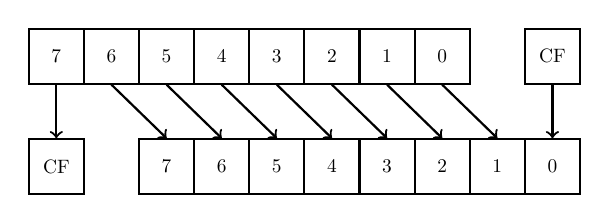
\begin{tikzpicture}[scale=0.7, every node/.style={scale=0.7}]
	\edef\bitsize{1cm}
	\tikzstyle{byte}=[draw,minimum size=\bitsize]
	\tikzstyle{every path}=[thick]

	\node [draw,rectangle,minimum size=\bitsize] (a1) {7};
	\node [draw,rectangle,minimum size=\bitsize] (a2) [right of=a1] {6};
	\node [draw,rectangle,minimum size=\bitsize] (a3) [right of=a2] {5};
	\node [draw,rectangle,minimum size=\bitsize] (a4) [right of=a3] {4};
	\node [draw,rectangle,minimum size=\bitsize] (a5) [right of=a4] {3};
	\node [draw,rectangle,minimum size=\bitsize] (a6) [right of=a5] {2};
	\node [draw,rectangle,minimum size=\bitsize] (a7) [right of=a6] {1};
	\node [draw,rectangle,minimum size=\bitsize] (a8) [right of=a7] {0};
	\node (empty1) [right of=a8] {};
	\node [rectangle,draw,minimum size=\bitsize] (acf) [right of=empty1] {CF};

	\node (empty) [below of=a1] {};

	\node [rectangle,draw,minimum size=\bitsize] (bcf) [below of=empty] {CF};
	\node (empty2) [right of=bcf] {};
	\node [draw,rectangle,minimum size=\bitsize] (b1) [right of=empty2] {7};
	\node [draw,rectangle,minimum size=\bitsize] (b2) [right of=b1] {6};
	\node [draw,rectangle,minimum size=\bitsize] (b3) [right of=b2] {5};
	\node [draw,rectangle,minimum size=\bitsize] (b4) [right of=b3] {4};
	\node [draw,rectangle,minimum size=\bitsize] (b5) [right of=b4] {3};
	\node [draw,rectangle,minimum size=\bitsize] (b6) [right of=b5] {2};
	\node [draw,rectangle,minimum size=\bitsize] (b7) [right of=b6] {1};
	\node [draw,rectangle,minimum size=\bitsize] (b8) [right of=b7] {0};

	\draw [->] (a1.south) -- (bcf.north); % 7
	\draw [->] (a2.south) -- (b1.north); % 6
	\draw [->] (a3.south) -- (b2.north);
	\draw [->] (a4.south) -- (b3.north);
	\draw [->] (a5.south) -- (b4.north);
	\draw [->] (a6.south) -- (b5.north);
	\draw [->] (a7.south) -- (b6.north);
	\draw [->] (a8.south) -- (b7.north);
	\draw [->] (acf.south) -- (b8.north);

	\end{tikzpicture}
\end{center}

  \item[RCR] (M) \RU{вращать биты направо через флаг CF}\EN{rotate right via CF flag}\FR{pivote vers la droite via le flag CF}:

\begin{center}
	\begin{tikzpicture}[scale=0.7, every node/.style={scale=0.7}]
	\edef\bitsize{1cm}
	\tikzstyle{byte}=[draw,minimum size=\bitsize]
	\tikzstyle{every path}=[thick]

	\node [rectangle,draw,minimum size=\bitsize] (acf) {CF};
	\node (empty1) [right of=acf] {};

	\node [draw,rectangle,minimum size=\bitsize] (a1) [right of=empty1] {7};
	\node [draw,rectangle,minimum size=\bitsize] (a2) [right of=a1] {6};
	\node [draw,rectangle,minimum size=\bitsize] (a3) [right of=a2] {5};
	\node [draw,rectangle,minimum size=\bitsize] (a4) [right of=a3] {4};
	\node [draw,rectangle,minimum size=\bitsize] (a5) [right of=a4] {3};
	\node [draw,rectangle,minimum size=\bitsize] (a6) [right of=a5] {2};
	\node [draw,rectangle,minimum size=\bitsize] (a7) [right of=a6] {1};
	\node [draw,rectangle,minimum size=\bitsize] (a8) [right of=a7] {0};

	\node (empty) [below of=a1] {};

	\node [draw,rectangle,minimum size=\bitsize] (b1) [below of=empty] {7};
	\node [draw,rectangle,minimum size=\bitsize] (b2) [right of=b1] {6};
	\node [draw,rectangle,minimum size=\bitsize] (b3) [right of=b2] {5};
	\node [draw,rectangle,minimum size=\bitsize] (b4) [right of=b3] {4};
	\node [draw,rectangle,minimum size=\bitsize] (b5) [right of=b4] {3};
	\node [draw,rectangle,minimum size=\bitsize] (b6) [right of=b5] {2};
	\node [draw,rectangle,minimum size=\bitsize] (b7) [right of=b6] {1};
	\node [draw,rectangle,minimum size=\bitsize] (b8) [right of=b7] {0};

	\node (empty2) [right of=b7] {};

	\node [rectangle,draw,minimum size=\bitsize] (bcf) [right=of empty2] {CF};

	\draw [->] (acf.south) -- (b1.north);
	\draw [->] (a1.south) -- (b2.north);
	\draw [->] (a2.south) -- (b3.north);
	\draw [->] (a3.south) -- (b4.north);
	\draw [->] (a4.south) -- (b5.north);
	\draw [->] (a5.south) -- (b6.north);
	\draw [->] (a6.south) -- (b7.north);
	\draw [->] (a7.south) -- (b8.north);
	\draw [->] (a8.south) -- (bcf.north);

	\end{tikzpicture}
\end{center}


\myindex{x86!\Instructions!ROL}
\myindex{x86!\Instructions!ROR}
\label{ROL_ROR}
\item[ROL/ROR] (M) décalage cyclique

ROL: rotation à gauche:

\input{rotate_left}

ROR: rotation à droite:

\input{rotate_right}

En dépit du fait que presque presque tous les \ac{CPU}s aient ces instructions, il n'y
a pas d'opération correspondante en \CCpp, donc les compilateurs de ces \ac{PL}s
ne génèrent en général pas ces instructions.

Par commodité pour le programmeur, au moins \ac{MSVC} fourni les pseudo-fonctions
(fonctions intrinsèques du compilateur)
\IT{\_rotl()} \AndENRU \IT{\_rotr()}\FNMSDNROTxURL{},
qui sont traduitent directement par le compilateur en ces instructions.


\myindex{x86!\Instructions!SAL}
  \item[SAL] \RU{Арифметический сдвиг влево}\EN{Arithmetic shift left}\FR{Décalager
  arithmétique à gauche}, \RU{синонимично}\EN{synonymous to}\FR{synonyme de} \TT{SHL}

\myindex{x86!\Instructions!SAR}
  \label{ins:SAR}
  \item[SAR] \RU{Арифметический сдвиг вправо}\EN{Arithmetic shift right}\FR{Décalage arithmétique à droite}

\begin{center}
	\begin{tikzpicture}[scale=0.7, every node/.style={scale=0.7}]
	\edef\bitsize{1cm}
	\tikzstyle{byte}=[draw,minimum size=\bitsize]
	\tikzstyle{every path}=[thick]

	\node [draw,rectangle,minimum size=\bitsize] (a1) {7};
	\node [draw,rectangle,minimum size=\bitsize] (a2) [right of=a1] {6};
	\node [draw,rectangle,minimum size=\bitsize] (a3) [right of=a2] {5};
	\node [draw,rectangle,minimum size=\bitsize] (a4) [right of=a3] {4};
	\node [draw,rectangle,minimum size=\bitsize] (a5) [right of=a4] {3};
	\node [draw,rectangle,minimum size=\bitsize] (a6) [right of=a5] {2};
	\node [draw,rectangle,minimum size=\bitsize] (a7) [right of=a6] {1};
	\node [draw,rectangle,minimum size=\bitsize] (a8) [right of=a7] {0};

	\node (empty) [below of=a1] {};

	\node [draw,rectangle,minimum size=\bitsize] (b1) [below of=empty] {7};
	\node [draw,rectangle,minimum size=\bitsize] (b2) [right of=b1] {6};
	\node [draw,rectangle,minimum size=\bitsize] (b3) [right of=b2] {5};
	\node [draw,rectangle,minimum size=\bitsize] (b4) [right of=b3] {4};
	\node [draw,rectangle,minimum size=\bitsize] (b5) [right of=b4] {3};
	\node [draw,rectangle,minimum size=\bitsize] (b6) [right of=b5] {2};
	\node [draw,rectangle,minimum size=\bitsize] (b7) [right of=b6] {1};
	\node [draw,rectangle,minimum size=\bitsize] (b8) [right of=b7] {0};

	\node [shape=rectangle,draw,minimum size=\bitsize] (cf) [right=of b7] {CF};

	\draw [->] (a1.south) -- (b1.north); %7
	\draw [->] (a1.south) -- (b2.north); %6

	\draw [->] (a2.south) -- (b3.north); %6
	\draw [->] (a3.south) -- (b4.north); %5
	\draw [->] (a4.south) -- (b5.north); %4
	\draw [->] (a5.south) -- (b6.north); %3
	\draw [->] (a6.south) -- (b7.north); %2
	\draw [->] (a7.south) -- (b8.north); %1

	\draw [->] (a8.south) -- (cf.north);

	\end{tikzpicture}
\end{center}

\RU{Таким образом, бит знака всегда остается на месте}%
\EN{Hence, the sign bit always stays at the place of the}%
\FR{De ce fait, le bit de signe reste toujours à la place du} \ac{MSB}.


\myindex{x86!\Instructions!SETcc}
  \item[SETcc] op: \RU{загрузить 1 в op (только байт) если условие верно или 0 если наоборот}%
  \EN{load 1 to operand (byte only) if the condition is true or zero otherwise}%
  \FR{charge 1 dans l'opérande (octet seulement) si la condition est vraie et zéro sinon}.
  \RU{Коды точно такие же, как и в инструкциях Jcc}\EN{The condition codes are the same as in the Jcc instructions}%
  \FR{Les codes conditions sont les même que les instructions Jcc}
  (\myref{Jcc}).


\myindex{x86!\Instructions!STC}
\myindex{x86!\Flags!CF}
  \item[STC] (M) \RU{установить флаг CF}\EN{set CF flag}\FR{met le flag CF}

\myindex{x86!\Instructions!STD}
\myindex{x86!\Flags!DF}
  \item[STD] (M) Met le flag DF.
   Cette instruction n'est pas générée par les compilateurs et est en général rare.
   Par exemple, elle peut être trouvée dans le fichier du noyau de Windows \TT{ntoskrnl.exe},
   dans la routine de copie mémoire écrite à la main.

\myindex{x86!\Instructions!STI}
\myindex{x86!\Flags!IF}
  \item[STI] (M) \RU{установить флаг IF}\EN{set IF flag}\FR{met le flag IF}

\myindex{x86!\Instructions!SYSCALL}
  \item[SYSCALL] (AMD) \RU{вызов сисколла}\EN{call syscall}\FR{appelle un appel système} (\myref{syscalls})

\myindex{x86!\Instructions!SYSENTER}
  \item[SYSENTER] (Intel) \RU{вызов сисколла}\EN{call syscall}\FR{appel un appel système} (\myref{syscalls})

\myindex{x86!\Instructions!UD2}
  \item[UD2] (M) \RU{неопределенная инструкция, вызывает исключение. Применяется для тестирования.}
  \EN{undefined instruction, raises exception. Used for testing.}\FR{instruction
  indéfinie, lève une exception. Utilisée pour tester.}

\myindex{x86!\Instructions!XCHG}
  \item[XCHG] (M) \RU{обменять местами значения в операндах}\EN{exchange the values in the operands}%
\FR{échange les valeurs dans les opérandes}

\myindex{Borland Delphi}
\RU{Это редкая инструкция: компиляторы её не генерируют, потому что начиная с Pentium, XCHG с адресом в памяти в операнде
исполняется так, как если имеет префикс LOCK (см.\InSqBrackets{\MAbrash глава 19}).
Вероятно, в Intel так сделали для совместимости с синхронизирующими примитивами.
Таким образом, XCHG начиная с Pentium может быть медленной.
С другой стороны, XCHG была очень популярна у программистов на ассемблере.
Так что, если вы видите XCHG в коде, это может быть знаком, что код написан вручную.
Впрочем, по крайней мере компилятор Borland Delphi генерирует эту инструкцию.}
\EN{This instruction is rare: compilers don't generate it, because starting at Pentium, XCHG with address in memory in operand executes as if it has LOCK prefix (\InSqBrackets{\MAbrash chapter 19}).
Perhaps, Intel engineers did so for compatibility with synchronizing primitives.
Hence, XCHG starting at Pentium can be slow.
On the other hand, XCHG was very popular in assembly language programmers.
So if you see XCHG in code, it can be a sign that this piece of code is written manually.
However, at least Borland Delphi compiler generates this instruction.}
\FR{Cette instruction est rare: les compilateurs ne la génère pas, car à partir du
Pentium, XCHG avec comme opérande une adresse en mémoire s'exécute comme si elle
avait le préfixe LOCK (\InSqBrackets{\MAbrash chapter 19}).
Peut-être que les ingénieurs d'Intel ont fait cela pour la compatibilité avec les
primitives de synchronisation.
Ainsi, à partir du Pentium, XCHG peut être lente.
D'un autre côté, XCHG était très populaire chez les programmeurs en langage d'assemblage.
Donc, si vous voyez XCHG dans le code, ça peut être un signe que ce morceau de code
a été écrit à la main.
Toutefois, au moins le compilateur Borland Delphi génère cette instruction.}


\end{description}

\subsubsection{Instructions FPU}

Le suffixe \TT{-R} dans le mnémonique signifie en général que les opérandes sont
inversés, le suffixe \TT{-P} implique qu'un élément est supprimé de la pile après
l'exécution de l'instruction, le suffixe \TT{-PP} implique que deux éléments sont
supprimés.

Les instructions \TT{-P} sont souvent utiles lorsque nous n'avons plus besoin que
la valeur soit présente dans la pile FPU après l'opération.

\begin{description}
\myindex{x86!\Instructions!FABS}
  \item[FABS] \RU{заменить значение в ST(0) на абсолютное значение ST(0)}\EN{replace value in ST(0) by absolute value in ST(0)}%
  \FR{remplace la valeur dans ST(0) par sa valeur absolue}

\myindex{x86!\Instructions!FADD}
\myindex{x86!\Instructions!FADDP}
  \item[FADD] op: ST(0)=op+ST(0)
  \item[FADD] ST(0), ST(i): ST(0)=ST(0)+ST(i)
  \item[FADDP] ST(1)=ST(0)+ST(1);
  \RU{вытолкнуть один элемент из стека, таким образом, складываемые значения в стеке заменяются
  суммой}\EN{pop one element from the stack, i.e., the values in the stack are replaced by their sum}%
  \FR{supprime un élément de la pile, i.e., les valeurs sur la pile sont remplacées par leurs somme}

 % + FADDP
\input{appendix/x86/instructions/FCHS}
\myindex{x86!\Instructions!FCOM}
\myindex{x86!\Instructions!FCOMP}
\myindex{x86!\Instructions!FCOMPP}
  \item[FCOM] compare ST(0) avec ST(1)
  \item[FCOM] op: compare ST(0) avec op
  \item[FCOMP] compare ST(0) avec ST(1); supprime un élément de la pile
  \item[FCOMPP] compare ST(0) avec ST(1); supprime deux éléments de la pile

 % + FCOMP + FCOMPP
\myindex{x86!\Instructions!FDIVR}
\myindex{x86!\Instructions!FDIVRP}
  \item[FDIVR] op: ST(0)=op/ST(0)
  \item[FDIVR] ST(i), ST(j): ST(i)=ST(j)/ST(i)
  \item[FDIVRP] op: ST(0)=op/ST(0); \RU{вытолкнуть один элемент из стека}\EN{pop one element from the stack}%
  \FR{supprime un élément de la pile}
  \item[FDIVRP] ST(i), ST(j): ST(i)=ST(j)/ST(i); \RU{вытолкнуть один элемент из стека}\EN{pop one element from the stack}%
  \FR{supprime un élément de la pile}

 % + FDIVRP
\myindex{x86!\Instructions!FDIV}
\myindex{x86!\Instructions!FDIVP}
  \item[FDIV] op: ST(0)=ST(0)/op
  \item[FDIV] ST(i), ST(j): ST(i)=ST(i)/ST(j)
  \item[FDIVP] ST(1)=ST(0)/ST(1); \RU{вытолкнуть один элемент из стека, таким образом,
  делимое и делитель в стеке заменяются частным}\EN{pop one element from the stack, i.e.,
  the dividend and divisor values in the stack are replaced by quotient}\FR{supprime un
  élément de la pile, i.e, les valeurs du dividende et du diviseur sont remplacées par
  le quotient}
 % + FDIVP
\myindex{x86!\Instructions!FILD}
  \item[FILD] op: \RU{сконвертировать целочисленный op и затолкнуть его в стек}
  \EN{convert integer and push it to the stack}\FR{convertit un entier n et le pousse sur la pile}.


\myindex{x86!\Instructions!FIST}
\myindex{x86!\Instructions!FISTP}
  \item[FIST] op: convertit  la valeur dansST(0) en un entier dans op
  \item[FISTP] op: convertit la valeur dans ST(0) en un entier dans op;
  supprime un élément de la pile
 % + FISTP
\myindex{x86!\Instructions!FLD1}
  \item[FLD1] \RU{затолкнуть 1 в стек}\EN{push 1 to stack}\FR{pousse 1 sur la pile}


\myindex{x86!\Instructions!FLDCW}
  \item[FLDCW] op: \RU{загрузить}\EN{load}\FR{charge le} FPU control word (\myref{FPU_control_word}) \RU{из}\EN{from}\FR{depuis le} 16-bit op.


\myindex{x86!\Instructions!FLDZ}
  \item[FLDZ] \RU{затолкнуть ноль в стек}\EN{push zero to stack}\FR{pousse zéro sur la pile}



\myindex{x86!\Instructions!FLD}
  \item[FLD] op: \RU{затолкнуть op в стек}\EN{push op to the stack}\FR{pousse op sur la pile}.

\myindex{x86!\Instructions!FMUL}
\myindex{x86!\Instructions!FMULP}
  \item[FMUL] op: ST(0)=ST(0)*op
  \item[FMUL] ST(i), ST(j): ST(i)=ST(i)*ST(j)
  \item[FMULP] op: ST(0)=ST(0)*op; \RU{вытолкнуть один элемент из стека}\EN{pop one element from the stack}%
  \FR{supprime un élément de la pile}
  \item[FMULP] ST(i), ST(j): ST(i)=ST(i)*ST(j); \RU{вытолкнуть один элемент из стека}\EN{pop one element from the stack}%
  \FR{supprime un élément de la pile}

 % + FMULP
\input{appendix/x86/instructions/FSINCOS}
\input{appendix/x86/instructions/FSQRT}
\myindex{x86!\Instructions!FSTCW}
\myindex{x86!\Instructions!FNSTCW}
  \item[FSTCW] op: stocker le mot de contrôle FPU (\myref{FPU_control_word}) dans l'op 16-bit
  après avoir vérifié s'il y a des exceptions en attente.
  \item[FNSTCW] op: stocker le mot de contrôle FPU (\myref{FPU_control_word}) dans l'op 16-bit.

 % + FNSTCW
\myindex{x86!\Instructions!FSTSW}
\myindex{x86!\Instructions!FNSTSW}
  \item[FSTSW] op: stocker le mot d'état FPU (\myref{FPU_status_word}) dans l'op 16-bit
  après avoir vérifié s'il y a des exceptions en attente.
  \item[FNSTSW] op: stocker le mot d'état FPU (\myref{FPU_status_word}) dans l'op 16-bit.

 % + FNSTSW
\myindex{x86!\Instructions!FST}
\myindex{x86!\Instructions!FSTP}
  \item[FST] op: \RU{копировать}\EN{copy}\FR{copie} ST(0) \RU{в}\EN{to}\FR{dans} op
  \item[FSTP] op: \RU{копировать}\EN{copy}\FR{copie} ST(0) \RU{в}\EN{to}\FR{dans} op;
  \RU{вытолкнуть один элемент из стека}\EN{pop one element from the stack}%
  \FR{supprime un élément de la pile}

\myindex{x86!\Instructions!FSUBR}
\myindex{x86!\Instructions!FSUBRP}
  \item[FSUBR] op: ST(0)=op-ST(0)
  \item[FSUBR] ST(0), ST(i): ST(0)=ST(i)-ST(0)
  \item[FSUBRP] ST(1)=ST(0)-ST(1);
  \RU{вытолкнуть один элемент из стека, таким образом, складываемые значения в стеке заменяются
  разностью}\EN{pop one element from the stack, i.e., the value in the stack is replaced by the difference}%
  \FR{supprime un élément de la pile, i.e., la valeur dans la pile est remplacée par la différence}

 % + FSUBRP
\myindex{x86!\Instructions!FSUB}
\myindex{x86!\Instructions!FSUBP}
  \item[FSUB] op: ST(0)=ST(0)-op
  \item[FSUB] ST(0), ST(i): ST(0)=ST(0)-ST(i)
  \item[FSUBP] ST(1)=ST(1)-ST(0);
  \RU{вытолкнуть один элемент из стека, таким образом, складываемые значения в стеке заменяются
  разностью}\EN{pop one element from the stack, i.e., the value in the stack is replaced by the difference}%
  \FR{supprime un élément de la pile, i.e., la valeur dans la pile est remplacée par la différence}

 % + FSUBP
\myindex{x86!\Instructions!FUCOM}
\myindex{x86!\Instructions!FUCOMP}
\myindex{x86!\Instructions!FUCOMPP}
  \item[FUCOM] ST(i): compare ST(0) \AndENRU ST(i)
  \item[FUCOM] compare ST(0) \AndENRU ST(1)
  \item[FUCOMP] compare ST(0) \AndENRU ST(1); supprime un élément de la pile.
  \item[FUCOMPP] compare ST(0) \AndENRU ST(1); supprime deux éléments de la pile.

  L'instruction se comporte comme FCOM, mais une exception est levée seulement si
  un opérande est SNaN, tandis que les nombres QNaN sont traités normalement.
 % + FUCOMP + FUCOMPP
\myindex{x86!\Instructions!FXCH}
  \item[FXCH] ST(i) \RU{обменять местами значения в ST(0) и ST(i)}\EN{exchange values in ST(0) and ST(i)}%
  \FR{échange les valeurs dans ST(0) et ST(i)}
  \item[FXCH] \RU{обменять местами значения в ST(0) и ST(1)}\EN{exchange values in ST(0) and ST(1)}%
  \FR{échange les valeurs dans ST(0) et ST(1)}


\end{description}

%\subsubsection{\RU{SIMD-инструкции}\EN{SIMD instructions}}

% TODO

%\begin{description}
%\input{appendix/x86/instructions/DIVSD}
%\input{appendix/x86/instructions/MOVDQA}
%\input{appendix/x86/instructions/MOVDQU}
%\input{appendix/x86/instructions/PADDD}
%\input{appendix/x86/instructions/PCMPEQB}
%\input{appendix/x86/instructions/PLMULHW}
%\input{appendix/x86/instructions/PLMULLD}
%\input{appendix/x86/instructions/PMOVMSKB}
%\input{appendix/x86/instructions/PXOR}
%\end{description}

% SHLD !
% SHRD !
% BSWAP !
% CMPXCHG
% XADD !
% CMPXCHG8B
% RDTSC !
% PAUSE!

% xsave
% fnclex, fnsave
% movsxd, movaps, wait, sfence, lfence, pushfq
% prefetchw
% REP RETN
% REP BSF
% movnti, movntdq, rdmsr, wrmsr
% ldmxcsr, stmxcsr, invlpg
% swapgs
% movq, movd
% mulsd
% POR
% IRETQ
% pslldq
% psrldq
% cqo, fxrstor, comisd, xrstor, wbinvd, movntq
% fprem
% addsb, subsd, frndint

% rare:
%\item[ENTER]
%\item[LES]
% LDS
% XLAT

\subsubsection{Instructions ayant un opcode affichable en ASCII\EN{Instructions having printable ASCII opcode}}

(En mode 32-bit).

\label{printable_x86_opcodes}
\myindex{Shellcode}
Elles peuvent être utilisées pour la création de shellcode.
Voir aussi: \myref{subsec:EICAR}.

% FIXME: break table
% FIXME: start at 0x20...
\begin{center}
\begin{longtable}{ | l | l | l | }
\hline
\HeaderColor caractère ASCII\EN{ character} & 
\HeaderColor code hexadécimal\EN{hexadecimal code} & 
\HeaderColor instruction x86\EN{ instruction} \\
\hline
0	 &30	 &XOR \\
1	 &31	 &XOR \\
2	 &32	 &XOR \\
3	 &33	 &XOR \\
4	 &34	 &XOR \\
5	 &35	 &XOR \\
7	 &37	 &AAA \\
8	 &38	 &CMP \\
9	 &39	 &CMP \\
:	 &3a	 &CMP \\
;	 &3b	 &CMP \\
<	 &3c	 &CMP \\
=	 &3d	 &CMP \\
?	 &3f	 &AAS \\
@	 &40	 &INC \\
A	 &41	 &INC \\
B	 &42	 &INC \\
C	 &43	 &INC \\
D	 &44	 &INC \\
E	 &45	 &INC \\
F	 &46	 &INC \\
G	 &47	 &INC \\
H	 &48	 &DEC \\
I	 &49	 &DEC \\
J	 &4a	 &DEC \\
K	 &4b	 &DEC \\
L	 &4c	 &DEC \\
M	 &4d	 &DEC \\
N	 &4e	 &DEC \\
O	 &4f	 &DEC \\
P	 &50	 &PUSH \\
Q	 &51	 &PUSH \\
R	 &52	 &PUSH \\
S	 &53	 &PUSH \\
T	 &54	 &PUSH \\
U	 &55	 &PUSH \\
V	 &56	 &PUSH \\
W	 &57	 &PUSH \\
X	 &58	 &POP \\
Y	 &59	 &POP \\
Z	 &5a	 &POP \\
\lbrack{}	 &5b	 &POP \\
\textbackslash{}	 &5c	 &POP \\
\rbrack{}	 &5d	 &POP \\
\verb|^|	 &5e	 &POP \\
\_	 &5f	 &POP \\
\verb|`|	 &60	 &PUSHA \\
a	 &61	 &POPA \\
f	 &66	 &en mode 32-bit, change pour une\EN{(in 32-bit mode) switch to}\\
   & & taille d'opérande de 16-bit\EN{16-bit operand size} \\
g	 &67	 &en mode 32-bit, change pour une\EN{(in 32-bit mode) switch to}\\
   & & taille d'adresse 16-bit\EN{16-bit address size} \\
h	 &68	 &PUSH\\
i	 &69	 &IMUL\\
j	 &6a	 &PUSH\\
k	 &6b	 &IMUL\\
p	 &70	 &JO\\
q	 &71	 &JNO\\
r	 &72	 &JB\\
s	 &73	 &JAE\\
t	 &74	 &JE\\
u	 &75	 &JNE\\
v	 &76	 &JBE\\
w	 &77	 &JA\\
x	 &78	 &JS\\
y	 &79	 &JNS\\
z	 &7a	 &JP\\
\hline
\end{longtable}
\end{center}

\myindex{x86!\Instructions!AAA}
\myindex{x86!\Instructions!AAS}
\myindex{x86!\Instructions!CMP}
\myindex{x86!\Instructions!DEC}
\myindex{x86!\Instructions!IMUL}
\myindex{x86!\Instructions!INC}
\myindex{x86!\Instructions!JA}
\myindex{x86!\Instructions!JAE}
\myindex{x86!\Instructions!JB}
\myindex{x86!\Instructions!JBE}
\myindex{x86!\Instructions!JE}
\myindex{x86!\Instructions!JNE}
\myindex{x86!\Instructions!JNO}
\myindex{x86!\Instructions!JNS}
\myindex{x86!\Instructions!JO}
\myindex{x86!\Instructions!JP}
\myindex{x86!\Instructions!JS}
\myindex{x86!\Instructions!POP}
\myindex{x86!\Instructions!POPA}
\myindex{x86!\Instructions!PUSH}
\myindex{x86!\Instructions!PUSHA}
\myindex{x86!\Instructions!XOR}

En résumé\EN{In summary}:
AAA, AAS, CMP, DEC, IMUL, INC, JA, JAE, JB, JBE, JE, JNE, JNO, JNS, JO, JP, JS, POP, POPA, PUSH, PUSHA, 
XOR.

 % subsection
\subsection{npad}
\label{sec:npad}

\RU{Это макрос в ассемблере, для выравнивания некоторой метки по некоторой границе.}
\EN{It is an assembly language macro for aligning labels on a specific boundary.}
\DE{Dies ist ein Assembler-Makro um Labels an bestimmten Grenzen auszurichten.}
\FR{C'est une macro du langage d'assemblage pour aligner les labels sur une limite
spécifique.}

\RU{Это нужно для тех \IT{нагруженных} меток, куда чаще всего передается управление, например, 
начало тела цикла. 
Для того чтобы процессор мог эффективнее вытягивать данные или код из памяти, через шину с памятью, 
кэширование, итд.}
\EN{That's often needed for the busy labels to where the control flow is often passed, e.g., loop body starts.
So the CPU can load the data or code from the memory effectively, through the memory bus, cache lines, etc.}
\DE{Dies ist oft nützlich Labels, die oft Ziel einer Kotrollstruktur sind, wie Schleifenköpfe.
Somit kann die CPU Daten oder Code sehr effizient vom Speicher durch den Bus, den Cache, usw. laden.}
\FR{C'est souvent necessaire pour des labels très utilisés, comme par exemple le
début d'un corps de boucle. Ainsi, le CPU peut charger les données ou le code depuis
la mémoire efficacement, à travers le bus mémoire, les caches, etc.}

\RU{Взято из}\EN{Taken from}\DE{Entnommen von}\FR{Pris de} \TT{listing.inc} (MSVC):

\myindex{x86!\Instructions!NOP}
\RU{Это, кстати, любопытный пример различных вариантов \NOP{}-ов. 
Все эти инструкции не дают никакого эффекта, но отличаются разной длиной.}
\EN{By the way, it is a curious example of the different \NOP variations.
All these instructions have no effects whatsoever, but have a different size.}
\DE{Dies ist übrigens ein Beispiel für die unterschiedlichen \NOP-Variationen.
Keine dieser Anweisungen hat eine Auswirkung, aber alle haben eine unterschiedliche Größe.}
\FR{À propos, c'est un exemple curieux des différentes variations de \NOP. Toutes
ces instructions n'ont pas d'effet, mais ont une taille différente.}

\RU{Цель в том, чтобы была только одна инструкция, а не набор NOP-ов, 
считается что так лучше для производительности CPU.}
\EN{Having a single idle instruction instead of couple of NOP-s,
is accepted to be better for CPU performance.}
\DE{Eine einzelne Idle-Anweisung anstatt mehrerer NOPs hat positive Auswirkungen
auf die CPU-Performance.}
\FR{Avoir une seule instruction sans effet au lieu de plusieurs est accepté comme
étant meilleur pour la performance du CPU.}

\begin{lstlisting}[style=customasmx86]
;; LISTING.INC
;;
;; This file contains assembler macros and is included by the files created
;; with the -FA compiler switch to be assembled by MASM (Microsoft Macro
;; Assembler).
;;
;; Copyright (c) 1993-2003, Microsoft Corporation. All rights reserved.

;; non destructive nops
npad macro size
if size eq 1
  nop
else
 if size eq 2
   mov edi, edi
 else
  if size eq 3
    ; lea ecx, [ecx+00]
    DB 8DH, 49H, 00H
  else
   if size eq 4
     ; lea esp, [esp+00]
     DB 8DH, 64H, 24H, 00H
   else
    if size eq 5
      add eax, DWORD PTR 0
    else
     if size eq 6
       ; lea ebx, [ebx+00000000]
       DB 8DH, 9BH, 00H, 00H, 00H, 00H
     else
      if size eq 7
	; lea esp, [esp+00000000]
	DB 8DH, 0A4H, 24H, 00H, 00H, 00H, 00H 
      else
       if size eq 8
        ; jmp .+8; .npad 6
	DB 0EBH, 06H, 8DH, 9BH, 00H, 00H, 00H, 00H
       else
        if size eq 9
         ; jmp .+9; .npad 7
         DB 0EBH, 07H, 8DH, 0A4H, 24H, 00H, 00H, 00H, 00H
        else
         if size eq 10
          ; jmp .+A; .npad 7; .npad 1
          DB 0EBH, 08H, 8DH, 0A4H, 24H, 00H, 00H, 00H, 00H, 90H
         else
          if size eq 11
           ; jmp .+B; .npad 7; .npad 2
           DB 0EBH, 09H, 8DH, 0A4H, 24H, 00H, 00H, 00H, 00H, 8BH, 0FFH
          else
           if size eq 12
            ; jmp .+C; .npad 7; .npad 3
            DB 0EBH, 0AH, 8DH, 0A4H, 24H, 00H, 00H, 00H, 00H, 8DH, 49H, 00H
           else
            if size eq 13
             ; jmp .+D; .npad 7; .npad 4
             DB 0EBH, 0BH, 8DH, 0A4H, 24H, 00H, 00H, 00H, 00H, 8DH, 64H, 24H, 00H
            else
             if size eq 14
              ; jmp .+E; .npad 7; .npad 5
              DB 0EBH, 0CH, 8DH, 0A4H, 24H, 00H, 00H, 00H, 00H, 05H, 00H, 00H, 00H, 00H
             else
              if size eq 15
               ; jmp .+F; .npad 7; .npad 6
               DB 0EBH, 0DH, 8DH, 0A4H, 24H, 00H, 00H, 00H, 00H, 8DH, 9BH, 00H, 00H, 00H, 00H
              else
	       %out error: unsupported npad size
               .err
              endif
             endif
            endif
           endif
          endif
         endif
        endif
       endif
      endif
     endif
    endif
   endif
  endif
 endif
endif
endm
\end{lstlisting}
 % subsection

